\documentclass{article}
\usepackage[]{multicol}
\usepackage{amsmath}
\usepackage{amssymb}
\usepackage{amsfonts}
\usepackage{listings}
\usepackage{graphicx}
\usepackage{caption}

\graphicspath{ {images/} }

% Reduce spacing
\usepackage[compact]{titlesec}
\titlespacing{\section}{0pt}{2ex}{1ex}
\titlespacing{\subsection}{0pt}{1ex}{0ex}
\titlespacing{\subsubsection}{0pt}{0.5ex}{0ex}
\usepackage{enumitem}
\setlist{nosep}
\setlength\parindent{0pt}


% Outer join symbols
\def\ojoin{\setbox0=\hbox{$\bowtie$}%
  \rule[-.02ex]{.25em}{.4pt}\llap{\rule[\ht0]{.25em}{.4pt}}}
\def\leftouterjoin{\mathbin{\ojoin\mkern-5.8mu\bowtie}}
\def\rightouterjoin{\mathbin{\bowtie\mkern-5.8mu\ojoin}}
\def\fullouterjoin{\mathbin{\ojoin\mkern-5.8mu\bowtie\mkern-5.8mu\ojoin}}

\usepackage[margin=12mm, landscape]{geometry}

\begin{document}
\begin{multicols*}{2}
    {\LARGE CS2102}
    \section*{Relational Algebra}
    $\sigma_{condition}(R)$ Select tuples from R that satisfy C eg. $\sigma_{a=b}(C)$\\
    Conditions:
    \begin{itemize}
        \item $\sigma_{a=1}(R)$
        \item $\sigma_{a=b}(R)$
        \item $\sigma_{a=1 \wedge/\vee b=2}(R)$
        \item $\sigma_{\neg (a=1)}(R)$

    \end{itemize}
    $\pi_{l}(R)$ Projects attributes from R in list $l$ eg. $\pi_{a,b}(C)$\\
    $p_{l}(R)$ Renames attributes from R \\
    Two formats: \\
    $p_{(a,b,c)}(A)$ renames them in order \\
    $p_{(a \leftarrow a1,b \leftarrow b1,c \leftarrow c1)}(A)$ renames a1 to a, b1 to b, c1 to c
    \subsection*{Set Operators}
    $A \cup B$\\ $A \cap B$\\ $A - B$ \\
    Cross Product: $A \times B$
    \subsection*{Inner Joins}
    $\theta-Join$ defined as $R \Join_\theta B = \sigma_{\theta}(R \times S)$\\
    Equi-Join defined as $\theta$-join with equal operator rather than other comparisons\\
    Natural Join $\Join$ joins over attributes that R and S have in common
    \subsection*{Outer Joins}
    $\leftouterjoin_\theta$ Left Outer Join: Inner join on $\theta$, then add dangling tuples (tuples from R that didn't join to any tuple from S)\\
    $\rightouterjoin_\theta$ Right Outer Join Same, but dangling tuples from S\\
    $\fullouterjoin_\theta$ Full Outer Join Same, but with all dangling tuples\\
    Natural outer joins exist too $\leftouterjoin \rightouterjoin \fullouterjoin$
    \section*{Relational Model}
    \begin{tabular}{|| c c ||}
        \hline
        Term            & Description                                            \\
        \hline\hline
        Superkey        & subset of attributes that uniquely identifies a tuple  \\
        (candidate) key & Minimal set of attributes that uniquely identify       \\
                        & a tuple in a relation                                  \\
        primary key     & Selected key (in case of multiple candidate keys)      \\
        foreign key     & Set of attributes that is a key in referenced relation \\
        prime attribute & Attribute of a primary key                             \\
        \hline
    \end{tabular}
    \section*{Constraints}
    \emph{Foreign Keys} must reference a primary key in another table (which can be itself).
    \section*{SQL}
    "x IS DISTINCT FROM y"
    \begin{itemize}
        \item equivalent to "x <> y" if x and y are non-null values
        \item if x and y both null $\rightarrow$ evaluates to false
        \item if only one value is null $\rightarrow$ evaluates to true
    \end{itemize}
    IS (NOT) NULL Comparison Predicate
    \begin{itemize}
        \item Check if a values is equal to null (since "=" would return unknown)
        \item If x is a null value $\rightarrow$ "x IS NULL" evaluates to true
        \item If x is a non-null value $\rightarrow$ "x IS NULL" evaluates to false    \end{itemize}
    \subsection*{Creating Tables}
    \begin{lstlisting}[language=SQL]
CREATE TABLE (
attribute INTEGER PRIMARY KEY
attribute2 TEXT REFERENCES table2(attribute2) NOT NULL
attribute3 INTEGER NOT NULL UNIQUE
attribute4 INTEGER constraint named_constraint
check(attribute4 > 5)
FOREIGN KEY (attribute3) REFERENCES table2(attribute3) 
ON DELETE action ON UPDATE action
)
    \end{lstlisting}
    Possible actions for on delete and on update:
    \begin{itemize}
        \item NO ACTION rejects delete/update if it violates constraint (default value)
        \item RESTRICT similar to "no action" except that check of constraint cannot be deferred
              (deferrable constraints are discussed in a bit)
        \item CASCADE propagates delete/update to referencing tuples
        \item SET DEFAULT updates foreign keys of referencing tuples to some default value
              (important: default value must be a primary key in the referenced table!)
        \item SET NULL updates foreign keys of referencing tuples to null
              (important: corresponding column must allowed to contain null values!)

    \end{itemize}
    \subsection*{Inserting Data}
    \begin{lstlisting}[language=SQL]
INSERT INTO Employees (id, name) 
VALUES (102, 'Judy'), (103, 'Max');
    \end{lstlisting}
    \subsection*{Updating Data}
    \begin{lstlisting}[language=SQL]
UPDATE Employees
SET age = age + 1
WHERE name = 'Sarah'; 
    \end{lstlisting}
    \subsection*{Deleting Data}
    \begin{lstlisting}[language=SQL]
DELETE FROM Employees 
WHERE role='dev';
    \end{lstlisting}
    \subsection*{Alter Table}
    \begin{lstlisting}[language=SQL]
ALTER TABLE Projects 
ALTER COLUMN start_year SET DEFAULT 2021; 
-- set default value of column "start_year"

ALTER TABLE Projects ALTER COLUMN start_year DROP DEFAULT;
-- drop default value of column "start_year"

ALTER TABLE Projects ALTER COLUMN name TYPE VARCHAR(200); 
-- change data type to VARCHAR(200)

ALTER TABLE Projects ADD COLUMN budget NUMERIC DEFAULT 0.0; 
-- add new column with a default value

ALTER TABLE Projects DROP COLUMN budget; 
-- drop column from table

ALTER TABLE Teams 
ADD CONSTRAINT eid_fkey FOREIGN KEY (eid)
REFERENCES Employees (id);

ALTER TABLE Teams DROP CONSTRAINT eid_fkey;
    \end{lstlisting}
    \section*{ERD}
    \subsection*{Attributes}
    \begin{itemize}
        \item specific information describing an entity
              represented by an oval in ER diagrams
    \end{itemize}
    4 subtypes of attributes
    \begin{itemize}
        \item Key attribute(s): uniquely identifies each entity (oval with the attribute name(s) underlines)
        \item Composite attribute: composed of multiple
              other attributes (oval comprising of ovals)
        \item Multivalued attribute: may consist of more
              than one value for a given entity (double-lined oval)
        \item Derived attribute: derived from other attributes
              (dashed oval)
    \end{itemize}
    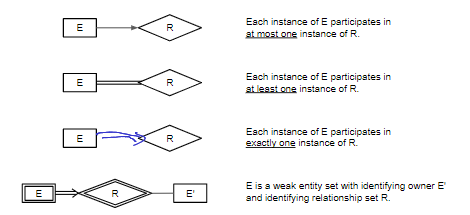
\includegraphics[scale=0.5]{summary_of_participation_constraints.png}
    \captionof{figure}{Summary of Participation Constraints}
    \subsection*{Implementations for constraints}
    Many A to Many B: Make a table A{\_}B that contains primary keys of both A and B\\
    One A to Many B: Put A's primary key in B\\
    One A to One B: Make a table A{\_}B that contains primary keys of both A and B as individually unique OR put one's primary key in the other table
    \subsection*{Weak Entity Set}
    Use primary key from identifying relation + another attribute as primary key
    Set ON DELETE CASCADE and ON UPDATE CASCADE
    \subsection*{Selecting}
    Basic pattern matching with (NOT) LIKE\\
    "{\_}" matches any single character\\
    "{\%}" matches any sequence of zero or more characters
    \begin{lstlisting}[language=SQL]
SELECT NAME FROM CITIES WHERE NAME LIKE 'Si%re'
SELECT NAME FROM CITIES WHERE NAME LIKE 'Si_re'
SELECT XX FROM XX WHERE XX.A IN ('A','B')
SELECT XX FROM XX WHERE XX.A < ANY/ALL (SELECT XX FROM XX)

SELECT xx FROM xx c1 WHERE xx >= ALL
 (SELECT XX from xx c2 WHERE c2.xx IS NOT NULL)
--need to check if not null else >= ALL will be false

SELECT A.X FROM A WHERE EXISTS 
    (SELECT B FROM C WHERE C.X = A.X)
--EXISTS

\end{lstlisting}
    \begin{lstlisting}[language=SQL]
SELECT name, population, gdp
FROM countries
WHERE ROW(population, gdp) > ANY (SELECT population, gdp
FROM countries
WHERE name IN ('Germany', 'France'))
--row constructor to compare two values, 
--if either is true it returns the row
\end{lstlisting}
    \subsection*{Recursive Queries}
    \begin{lstlisting}[mathescape=true]
WITH RECURSIVE cte_name AS (
    $Q_1$
    UNION [ ALL ]
    $Q_2$(cte_name)
)
SELECT * FROM cte_name
\end{lstlisting}
    {\large Example:}
    \begin{lstlisting}[language=SQL]
WITH RECURSIVE flight_path AS (
    SELECT from_code, to_code, 0 AS stops
    FROM connections
    WHERE from_code = 'SIN'
    UNION ALL
    SELECT c.from_code, c.to_code, p.stops+1
    FROM flight_path p, connections c
    WHERE p.to_code = c.from_code
    AND p.stops < 2
)
SELECT DISTINCT to_code, stops
FROM flight_path
ORDER BY stops ASC
\end{lstlisting}
    \subsection*{ISA}
    If A ISA B, put foreign key in A that references B\\
    Covering constraint: True if A needs to be at least a B
    Overlap constraint: True if A can be more than one B\\
    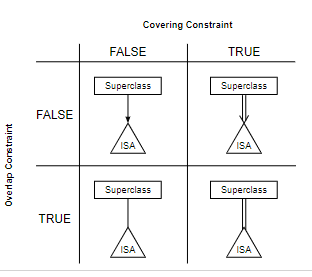
\includegraphics{ISA constraints.png}
    \subsection*{Aggregation}
    Treat relationship as entity, make a table Relationship-Entity with primary keys of the relationship and the entity as the primary key\\
    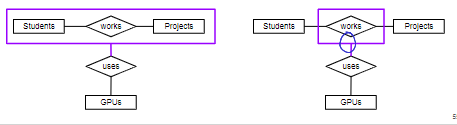
\includegraphics{aggregation.png}
\end{multicols*}
\end{document}
